% !TeX root = ../DCR-Consensus.tex
% !TeX spellcheck = en_GB
\chapter{Domain Analysis}
\label{chap:domainanalysis}

\section{What is a History}
\begin{definition}
	An \textit{\textbf{Action}}\index{Action|(} contains the following information:
	\begin{itemize}
		\item The Id of the source Event, this is the Event that has logged the action.
		\item The time stamp of the action local to the source Event.
		\item The Id of the participating Event, this is the Event that are being contacted, or the Event who has initiated the action.
		\item The type of the Action, i.e. \texttt{IncludedBy}.
	\end{itemize}
	
	The reason that an Action is not called Event\index{Event}, is because this term is used for an Event in the DCR Graph workflow.
	\index{Action|)}
\end{definition}

\begin{definition}\label{definition:historya}
	A \textit{\textbf{History}}\index{History} is a set of Actions.\index{Action}
\end{definition}

\begin{lemma}\label{lemma:partialorder}
	A set is in partial order if the relation between elements in the set is reflexive, antisymmetric, and transitive.
	If S is a partially ordered set and every two elements of S are comparable, S is called a totally ordered or linearly ordered set, and the relation between elements in the set is a total or linear order.
	\todo[inline]{Source: Discrete Mathematics and its Applications, 7th ed. - Kenneth H. Rosen - Afsnit 9.6, Partial Orderings}
	
	\newpar If Action $A$ has timestamp $a$, Action $B$ has timestamp $b$ and Action $C$ has timestamp $c$ in the local history H, and $a \geq a$ for every timestamp $a$, the relation $\geq$ is reflexive. If $a \geq b$ and $b \geq a$, then $a = b$. Therefore the relation $\geq$ is antisymmetric. Finally, $\geq$ is transitive because $a \geq b$ and $b \geq c$ imply that $a \geq c$. It follows that $\geq$ is a partial ordering on the set of timestamps. The same properties are present for $\leq$. 
	
	\newpar A local history is therefore totally ordered since the source Event knows the timestamps of all Actions, and the relation between timestamps of Actions is reflexive, antisymmetric and transitive. 
	
	\newpar In a workflow these local histories are put together. This creates the possibility of having histories that cannot be totally ordered, because there haven't been exchanged messages between the source Events between the actions.\todo{Dette forstår jeg ikke. - Fisk} This means that it is not possible to decide between all pairs of actions, which action happened first.
	
	There is one limitation on the order of the actions that must be fulfilled by any history, locally or globally. That is, that the history cannot contain cycles as this would imply that two (or more) actions would have to happen before the other.
	
	\todo[inline]{Lav et argument, eller find nogle andre der har defineret at en total order også er en partial order. (I forhold til Wiki-definitionen ovenfor, er det er en partial order ikke har den 3. begrænsning, men at det ellers er det samme, og derfor er partial order en svagere definition af total order.)}
	
	This creates the need for a history of partial order.
\end{lemma}

\newpar Because of \autoref{lemma:partialorder} we can update \autoref{definition:historya} to the following definition:

\begin{definition}
	A \textit{\textbf{History}}\index{History} is a \textit{partially ordered} set of Actions.\index{Action}
	\label{definition:historyb}
\end{definition}

\section{Relations between logs}
\label{sec:relations}
All logs have the form (\#Number, FromID, RelationType, ToID/ByID)
\subsection{Inclusion}
\begin{tabularx}{\textwidth}{|*{3}{>{\raggedright\arraybackslash}X|}}
  \hline
  Relation & Event1 Log & Event2 Log \\
  \hline
  Event 1 includes Event 2 & (\#1, Event 1, includes, Event 2) & (\#1, Event 2, includedBy, Event 1) \\
  \hline
  Event 2 includes Event 1 & (\#1, Event 1, includedBy, Event 2) & (\#3, Event 2, includes, Event 1) \\
  \hline
\end{tabularx}

\subsection{Exclusion}

\begin{tabularx}{\textwidth}{|*{3}{>{\raggedright\arraybackslash}X|}}
  \hline
  Relation & Event1 Log & Event2 Log \\
  \hline
  Event 1 excludes Event 2 & (\#1, Event 1, excludes, Event 2) & (\#1, Event 2, excludedBy, Event 1) \\
  \hline
  Event 2 excludes Event 1 & (\#1, Event 1, excludedBy, Event 2) & (\#3, Event 2, excludes, Event 1) \\
  \hline
\end{tabularx}

\subsection{Pending}
\begin{tabularx}{\textwidth}{|*{3}{>{\raggedright\arraybackslash}X|}}
  \hline
  Relation & Event1 Log & Event2 Log \\
  \hline
  Event 1 sets Pending Event 2 & (\#1, Event 1, setsPending, Event 2) & (\#1, Event 2, setPendingBy, Event 1) \\
  \hline
  Event 2 sets Pending Event 1 & (\#1, Event 1, setPendingBy, Event 2) & (\#3, Event 2, setsPending, Event 1) \\
  \hline
\end{tabularx}

\subsection{Conditions}
\begin{tabularx}{\textwidth}{|*{3}{>{\raggedright\arraybackslash}X|}}\hline
	Relation & Event1 Log & Event2 Log \\\hline
	Event 1 checks Event 2 which is executable & (\#1, Event 1, ConditionChecks true, Event 2) & (\#1, Event 2, ConditionChecked true, Event 1) \\\hline
	Event 1 checks Event 2 which is not executable & (\#1, Event 1, ConditionChecks false, Event 2) & (\#3, Event 2, ConditionChecked false, Event 1) \\\hline
	Event 2 checks Event 1 which is executable & (\#1, Event 1, ConditionChecked true, Event 2) & (\#1, Event 2, ConditionChecks true, Event 1) \\\hline
	Event 2 checks Event 1 which is not executable & (\#1, Event 1, ConditionChecked false, Event 2) & (\#3, Event 2, ConditionChecks false, Event 1) \\\hline
\end{tabularx}

\subsection{Execution}
\begin{tabularx}{\textwidth}{ | X | X | }
  \hline
  Relation & Event1 Log \\
  \hline
  Event 1 Execution begins & (\#1, Event 1, executionStart, ClientID) \\
  \hline
  Event 1 Execution fails & (\#2, Event 1, executionFail, ClientID) \\
  \hline
  Event 1 Execution success & (\#2, Event 1, executionSuccess, ClientID) \\
  \hline
\end{tabularx}

\subsection{Lock}
\begin{tabularx}{\textwidth}{|*{3}{>{\raggedright\arraybackslash}X|}}
  \hline
  Relation & Event1 Log & Event2 Log \\
  \hline
  Event 1 Locks Event 2 & (\#1, Event 1, lock, Event 2) & (\#1, Event 2, lockedBy, Event 1) \\
  \hline
  Event 2 Locks Event 1 & (\#1, Event 1, lockBy, Event 2) & (\#3, Event 2, lock, Event 1) \\
  \hline
\end{tabularx}

\subsection{Unlock}
\begin{tabularx}{\textwidth}{|*{3}{>{\raggedright\arraybackslash}X|}}
  \hline
  Relation & Event1 Log & Event2 Log \\
  \hline
  Event 1 Locks Event 2 & (\#1, Event 1, unlock, Event 2) & (\#1, Event 2, unlockedBy, Event 1) \\
  \hline
  Event 2 Locks Event 1 & (\#1, Event 1, unlockBy, Event 2) & (\#3, Event 2, unlock, Event 1) \\
  \hline
\end{tabularx}

\section{Happens Before Relations}

\begin{lstlisting}[breaklines=true]
    Y includedBy X       ->    X includes Y
    Y excludedBy X       ->    X excludes Y
    Y setPendingBy X     ->    X setsPending Y
    Y ConditionChecked X ->    X ConditionChecks Y
    Y LockedBy X         ->    X Lock Y
    Y UnlockedBy X       ->    X Unlock Y
    X Execution begins   ->    X Execution fails / Success
    X Execute Start      ->    X Locks Y
    X Locks Y            ->    X Include Y
    X Locks Y            ->    X Exclude Y
    X Locks Y            ->    X setPending Y
    X Locks Y            ->    X ConditionChecks Y
    X Locks Y            ->    X Unlock Y
    X Locks Y            ->    X Unlock Y     ->    X Execute Fail / Success
    Y Lockby X           ->    Y UnlockBy X   ->    Y LockBy "z"
\end{lstlisting}

\section{Malicious Nodes}
We assume that a malicious event can cheat in the following three ways.
\begin{definition}\label{malevent-type-omit}
	A malicious \texttt{event} can omit \texttt{logs} when asked for its \texttt{history}.
\end{definition}
\begin{definition}\label{malevent-type-add}
	A malicious \texttt{event} can add none-existent, consistent or inconsistent \texttt{logs} when asked for its \texttt{history}.
\end{definition}
\begin{definition}\label{malevent-type-responddifferent}
	A malicious \texttt{event} can send different \texttt{histories} to different requests.
\end{definition}
Furthermore we must assume that the first contacted event is not malicious, since if it is and returns faulty information there is no way to discover and recover from this. 

\newpar Creating history in a DCR graph with malicious events has similar characteristics as that of the Byzantine generals problem, described by Lamport e.l. in \todo{ref}. Each of these situations have some distributed systems, in which data has to be passed around and reached consensus about. Though creating a history has some differences, that must be worked around to apply the Byzantine generals algorithm to ensure consensus, we can argue that the algorithms proposed for the Byzantine generals problem still can be used. The first difference is that in DCR-graphs a single event do not propose a singular value to get consensus about, but must gather values from each event in the graph since each event is the only one who is knows the value for it self. To argue that this does not change the problem domain, we see the information gathering process from the perspective of the requested event instead of the requester. The situation is now similar to that of the Byzantine generals because the requested event returns and therefore propose a value that all of its requesters have to agree and get consensus on.

\newpar If we assume that the domain is a Byzantine generals problem, the same properties must exist in the DCR graph and we can therefore say that for a DCR graph to reach consensus on a history we need 3m+1 events with a maximum of m malicious events, when the DCR graph represents a 3-regular graph where there exist a path from loyal \texttt{event I} to any loyal \texttt{event k}.

%Gammel argumentation
We need to argue that all DCR graphs can be built using a group of base structures. Each of these base structures have properties which can be used to describe the safety of the DCR graph history:

\begin{figure}[H]
	\centering
	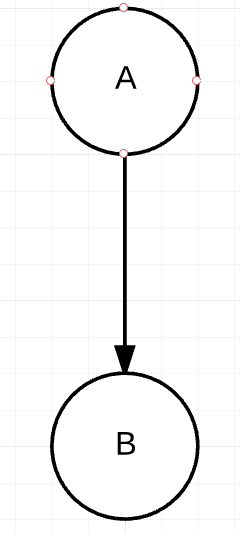
\includegraphics[height=5cm]{figures/GraphStructure_OneToOne}
	\caption{With a maximum of one malicious event in this graph structure and it not being event $A$, we have no way of telling if $B$ lies or not.}
\end{figure}
\todo[inline]{Figur har underlige prikker på Event A.}

\begin{figure}[H]
	\centering
	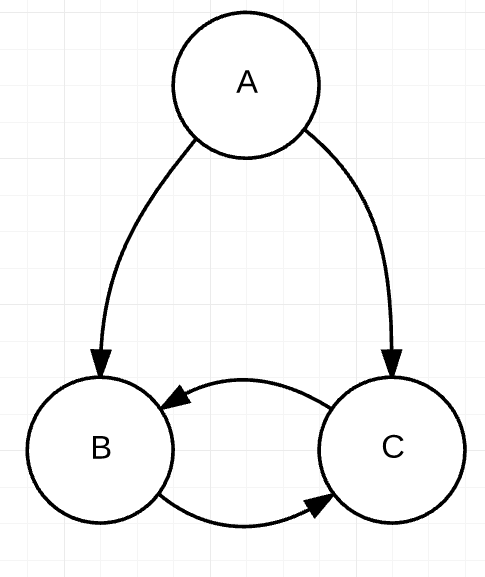
\includegraphics[height=5cm]{figures/GraphStructure_OneToTwo}
	\caption{With a maximum of one malicious event in this graph structure and it not being event $A$, we are able to determine that someone lies but not who.}
\end{figure}

\begin{figure}[H]
	\centering
	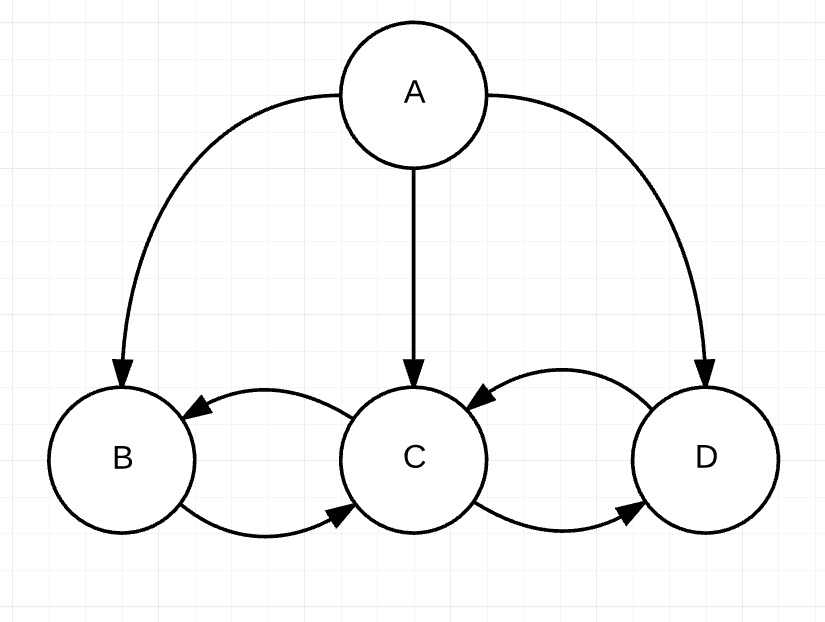
\includegraphics[height=5cm]{figures/GraphStructure_OneToTwoChain}
	\caption{This graph is just an extension of that above and therefore proposes the same properties.}
\end{figure}

\begin{figure}[H]
	\centering
	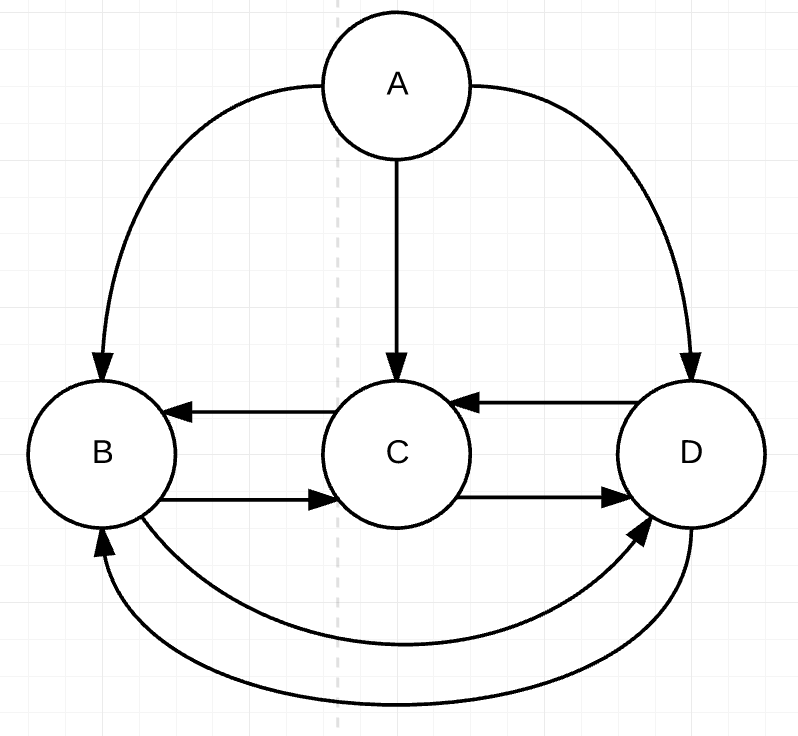
\includegraphics[height=5cm]{figures/GraphStructure_OneToThree}
	\caption{With a maximum of one malicious event in this graph structure and it not being event $A$, we are able to determine that someone lies and who lies.}
\end{figure}

\newpar With these base structures it is possible to strengthen the requirements of the DCR graph to not only require that a maximum $M$ amount of malicious events exist is in a graph with $3M+1$ events (taken from the byzantine generals problem\todo{Source? - Fisk}). To use these rules, we must therefore have a maximum of 1 malicious events in each of these subgraphs.

\chapter{Algorithms}
The overall problem is: given a DCR graph with possible malicious nodes, for the events of the graph to reach consensus of a partial order of execution that has happened in that graph.

The algorithm consists of the following sub-algorithms executed in the following order:
\begin{itemize}
    \item Produce - gathers the history.
    \item Elect - checks if the majority of the workflow can accept the proposed history
    \item Simplify - takes the history and creates an order of execution.
\end{itemize}

\newpar Correctness should be based on:
\begin{itemize}
    \item How many events are corrupted.
    \item How well the algorithm can determine which events are corrupted.
    \item How well the algorithm can determine if any and how many events are corrupted.
\end{itemize}

%History is created by using Fetch-and-Stitch with validation in the stitching phase.

%The receiver of the first create history call should

%- create history ID
%- fetch history from neighbours
%    - each of these should:
%        - fetch
%        - stitch
%        - return
%- stitch
%- Call for a vote
%- Closure of event graph to an execution graph.
\section{Data Structure}\label{sec:datastructure}
\todo[inline]{Retfærdiggør valget af datastruktur.}
\begin{lstlisting}[breaklines=true]
type Node {
	Id: EventId + Local TimeStamp;
	Type: String or Relation type;
	... more information about the log entry ...
	Edges: Node.Id list;
}

type Graph {
	Nodes: Map<Node.Id, Node>	- evt. Map<Node.Id, (Node * Node.Id list)
}
\end{lstlisting}
% !TeX root = ../DCR-Consensus.tex
\section{Stitch}
\subsection{Analysis} % Hvad er problemet
\subsection{Implementation} % hvordan løses det
\subsection{Discussion} % bliver problemet løst
\subsection{Performance} % hvor godt løses det


% !TeX root = ../DCR-Consensus.tex
\section{Produce}
\subsection{Goal} % Hvad er problemet
The goal of the algortithm is, given a DCR graph, to fetch and merge the histories of each event in the graph into one history, such that the resulting history is partially ordered in accordance to the ruleset described in \autoref{chap:domainanalysis}. 

%Correcness should be based on:
%\begin{itemize}
%    \item How many nodes' history gets fetched in the workflow (higher is better).
%    \item How rendundant the data is (higher redundancy is better).
%    \item How well it handles cycles in the graph
%\end{itemize}

\subsection{Implementation} % hvordan løses det
The implementation of the algorithm starts at a single event in the workflow and is called recursively on the reachable events in the workflow. A reachable event in the workflow constitutes any event that has a relation from the current event in scope. \todo[inline]{Udvid beskrivelse til at inkludere løsning hvis event peger på nuværende event. Dette event er p.t. ikke "synligt".}


\begin{lstlisting}[breaklines=true]
 1. History is requested by `X` with `request trace` `T` and history ID: `HID`
    1. If (Lookup history for `HID`) is not empty
        - Return lookup history for `HID`
    - Add all relations to `wait for`
    - If `wait for` is empty
        - Create history
        - Return
    - For each node `n` in `T`
        - if `n` is in `wait for`
            - remove `n` from `wait for`
    - Create `T'` by appending own ID to `T`
    - If `wait for` is empty
        - Cyclic case: Return empty set -> maybe return local set
    - Ask all nodes in `wait for` for their history with `T'`
    - Stitch own history with answers
    - Return "new" history
\end{lstlisting}

\subsection{Discussion} % bliver problemet løst
\subsection{Performance} % hvor godt løses det
% !TeX root = ../DCR-Consensus.tex
% !TeX spellcheck = en_GB
\section{Elect}
\subsection{Goal} % Hvad er problemet
The goal of the algorithm is, given a partially ordered history, to reach consensus upon the history between the participating events of the history.

\subsection{Implementation}
Since the partially ordered history includes URIs to all the events of the system, the initiator of the history call can contact all events who have contributed to the history. By sending the history to all the contributing events, each of them can send back an Accept or Reject call, thereby having an election on the created history. Then according to the regular rules of distributed system elections, if the majority accepts the proposed value, and no more than a third of the events are byzantine the election can be accepted, and returned.
\todo[inline]{Source: An Optimal Probabilistic Protocol For Synchronous Byzantine Agreement - Pesech Feldman \& Silvio Micali - http://bit.ly/1Q30qAC} 

\subsection{Discussion} % bliver problemet løst
\subsection{Performance}
Requires \texttt{2N} calls where \texttt{N} is the number of events in the system.


% !TeX root = ../DCR-Consensus.tex
\section{Simplify}
\subsection{Goal} % Hvad er problemet
The goal of the algorithm is, given a partially ordered history, to create an order of execution, where execution is a particular form of log.
\todo{maybe do the problem description polymorphic}

\subsection{Implementation} % hvordan løses det
\begin{algorithmic}
	\State \Comment{Find start nodes}
	\ForAll{node in graph}
	    \If{node has no incoming edge}
		    \State add to startFromSet
		\EndIf
	\EndFor
	
	\State \Comment{Create transitive clousures}
	\ForAll{node1 in startFromSet}
	    \ForAll{edge to node2}
	        \If {node2 is execution log}
	            \State add edge from node1 to node2
	            \State add node2 to startFromSet
	            \State break
	        \EndIf
	    \EndFor
	\EndFor
	
	\State \Comment{Remove all non execution logs}
	\ForAll{node in graph}
	    \If {not execution log}
	        \State remove node from graph
	    \EndIf
	\EndFor
	      
	\State \Comment{Transitive reduction}
	\ForAll{node1 in graph}
	  \ForAll{node2 in graph}
	    \If{edge between node1 and node2 exists}
	      \ForAll{node3 in graph}
	        \If{edge between node1 and node3 exists}
	          \State remove node from node1 to node3
	        \EndIf
	      \EndFor
	    \EndIf
	  \EndFor
	\EndFor
\end{algorithmic}
\subsection{Discussion} % bliver problemet løst
\subsection{Performance} % hvor godt løses det


